\documentclass[thesis.tex]{subfiles}
\renewcommand\_{\textunderscore\allowbreak}

\begin{document}


\chapter{ISR Correction}

The initial state radiation (ISR) can boost the total transverse energy of the hard scattering and affect kinematic quantities like object $p_T$ or $p_T^{miss}$.  In the case of the V+$\gamma$ process, we observed a systematic discrepancy between the data and simulation at high photon $p_T$. To improve the agreements between data and Madgraph samples, we reweight the MC events with correction factors derived from the analysis of $Z\gamma\rightarrow \mu\mu\gamma$ events.

The same MuonEG dataset and HLT\_MuEG triggers are used to select events with one photon and exactly two isolated muons.  The leading muon and the photon should pass the crteria deifned in Section 3, and the sub-leading muon is required to have $p_T >$ 15 GeV. In addition, the di-muon mass is required to be between 80 and 100 GeV. The ISR $p_T$ is deifned as the vector sum of all jets which have $p_T >$ 30 GeV and $|\eta| <$ 2.5.  To avoid counting the decays products of the Z boson, the jets are cleaned from isolated leptons. Contributions of fake photons are estimated and removed using the same methods described in  Section4.2.  Other rare backgrounds, including $t\bar{t}\gamma$, WWG and WZG are estimated using MC sampels.

Figure \ref{fig:apen-ISRJetPt} shows the comparision between the ISR $p_T$ spectrum of the data and simulation. The simulation over-predicts the number of events at high pt by about 35\%. The data-to-MC ratio in coarse pt bins are taken as the correction factors, as shown in \ref{table:apen-ISR}. We reweight the WG and ZG samples event-by-event using the ISR correction factors while keeping the total normalization unchanged. The ISR reweighting simultaneously improves the modeling of multiple variables, including photon $p_T$, $p_T^{miss}$ and $M_T$, as shown in Figure \ref{fig:apen-withcorr}.

\begin{table}[htdp]
	\centering
  \begin{tabular}{|c|c|}
  \hline
	ISR $p_T$ (GeV)& Correction $\pm$ stat. unc. $\pm$ syst. unc.\\ \hline
  0-50           & 1.015 $\pm$ 0.018 $\pm$ 0.04\\ \hline
  50-100         & 1.110 $\pm$ 0.015 $\pm$ 0.03\\ \hline
  100-150        & 0.845 $\pm$ 0.023 $\pm$ 0.04\\ \hline
  150-200        & 0.715 $\pm$ 0.035 $\pm$ 0.07\\ \hline
  200-250        & 0.730 $\pm$ 0.056 $\pm$ 0.09\\ \hline
  250-300        & 0.732 $\pm$ 0.086 $\pm$ 0.08\\ \hline
  $>$ 300        & 0.642 $\pm$ 0.069 $\pm$ 0.08\\ \hline
  \end{tabular}
  }
  \caption{Correction factors for the ISR reweighting.}
  \label{table:apen-ISR}
\end{table}


\begin{figure}
  \centering
    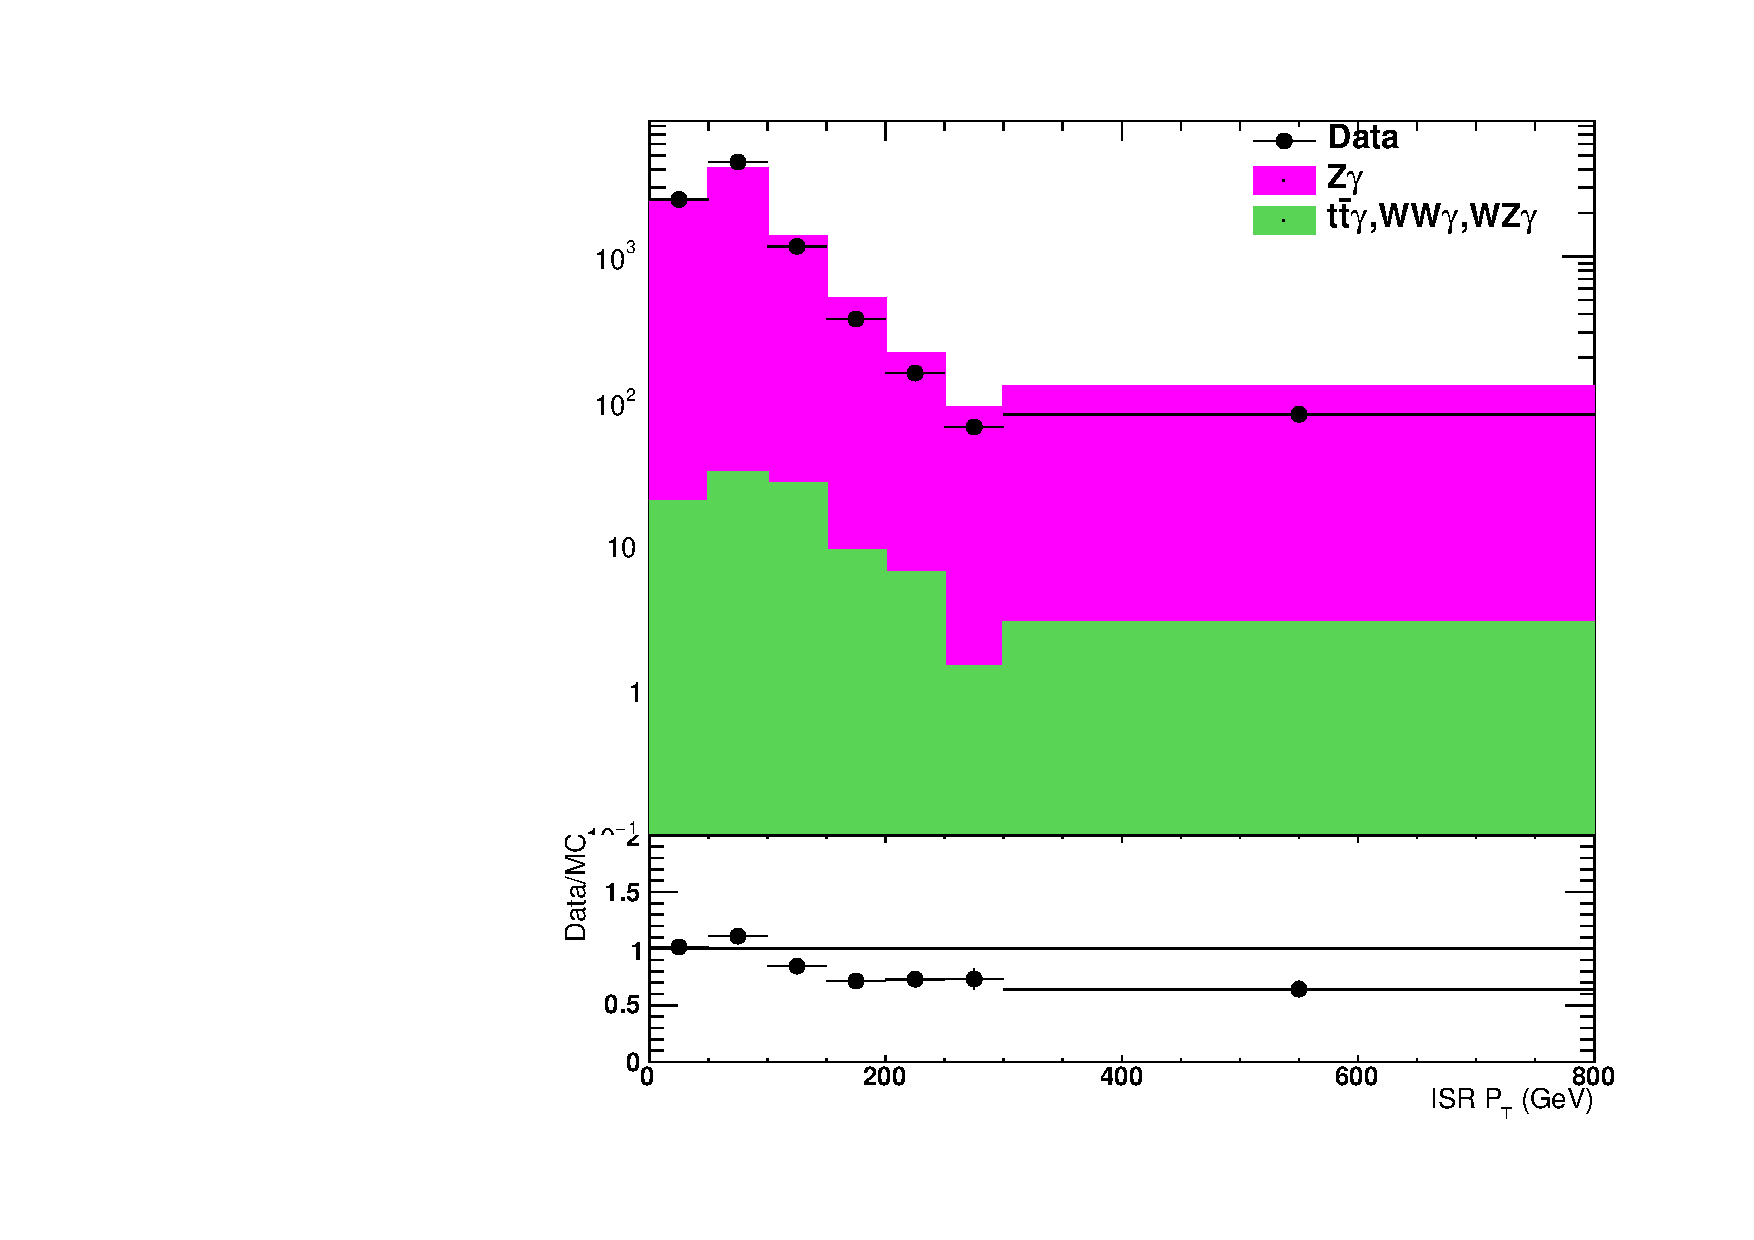
\includegraphics[width=0.5\textwidth]{Figures/PLOT_ISRweight.pdf}
  \caption{The electron misidentification rate as a function of $p_T$ (top left), $\eta$ (top right) and $N_{vtx}$ (bottom), along with the systematic uncertainties.}
  \label{fig:apen-ISRJetPt}
\end{figure}


\begin{figure}
  \centering
    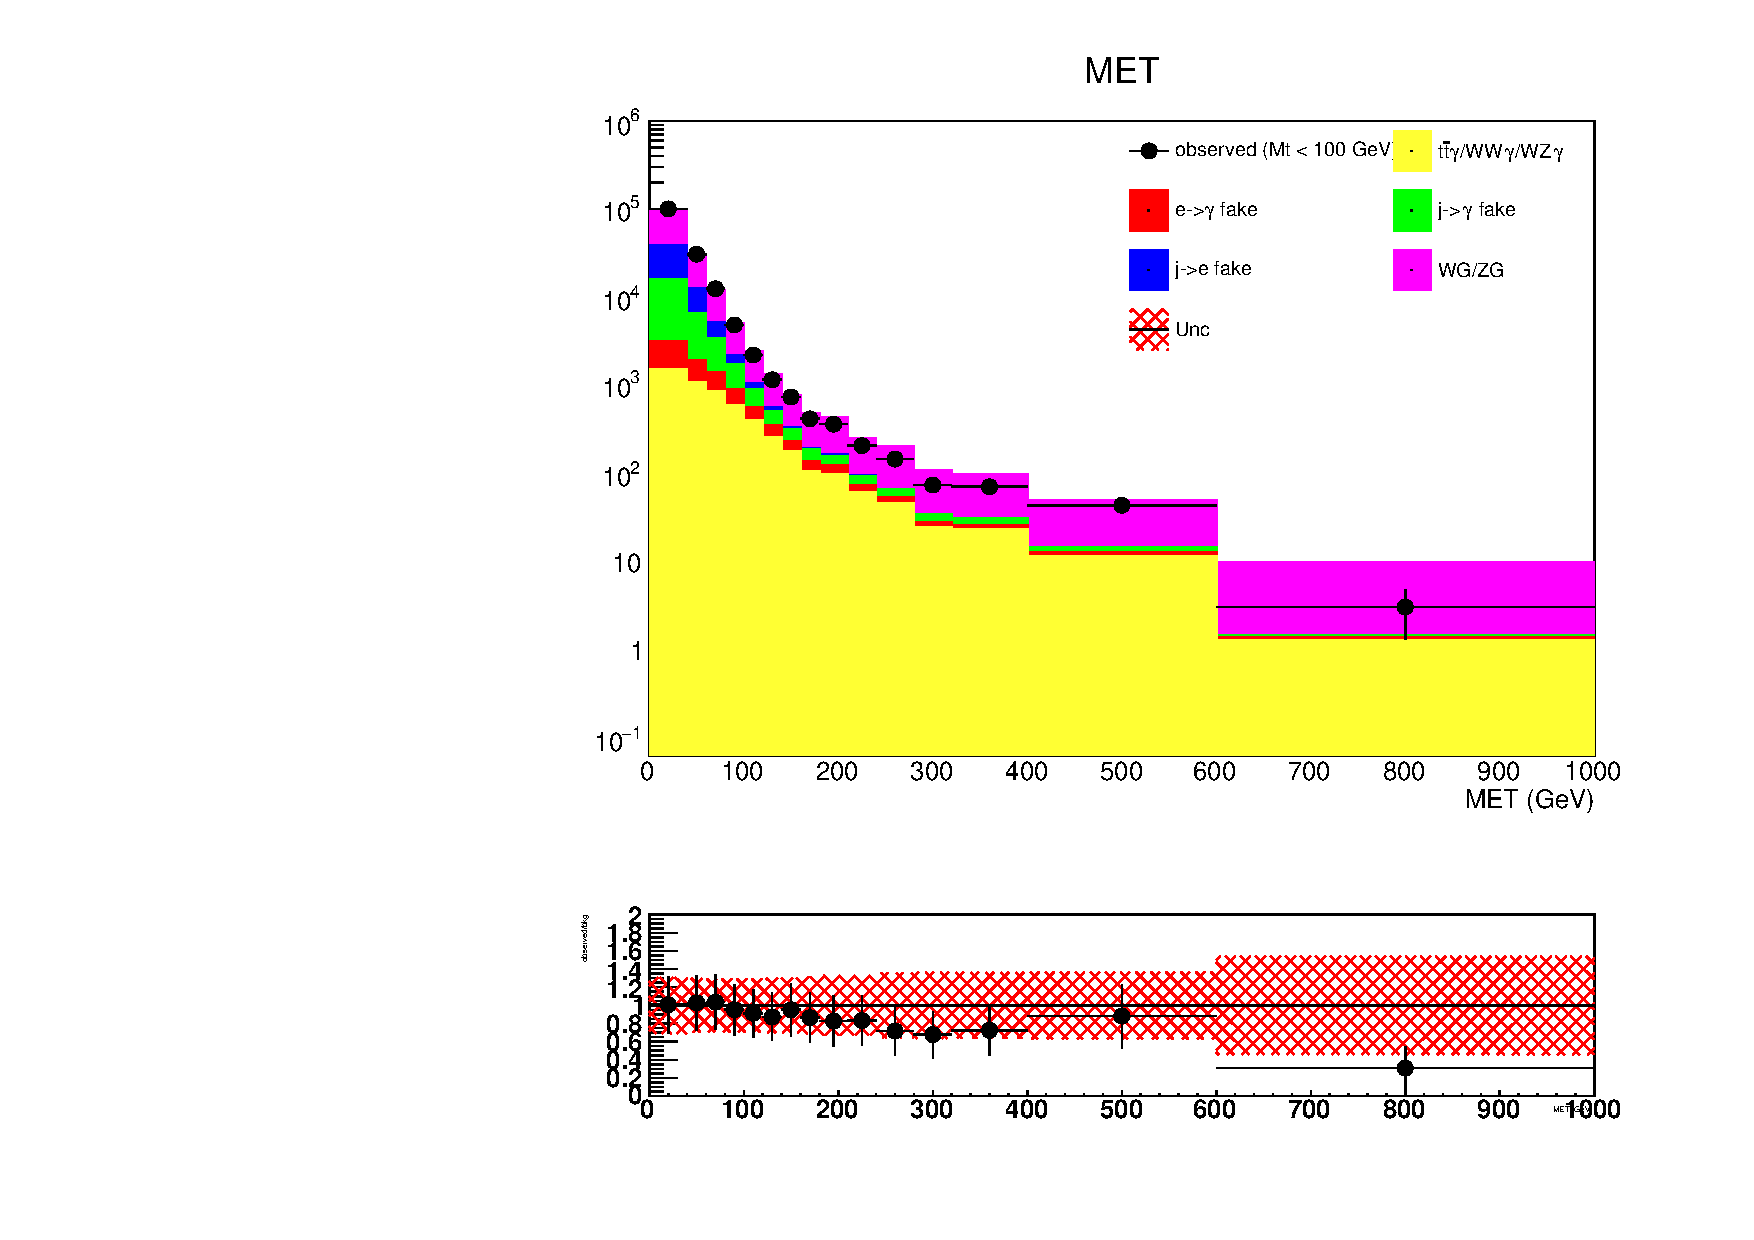
\includegraphics[width=0.45\textwidth]{Figures/VALIDNOCOR_mg_2016ReMiniAOD_met.pdf}
    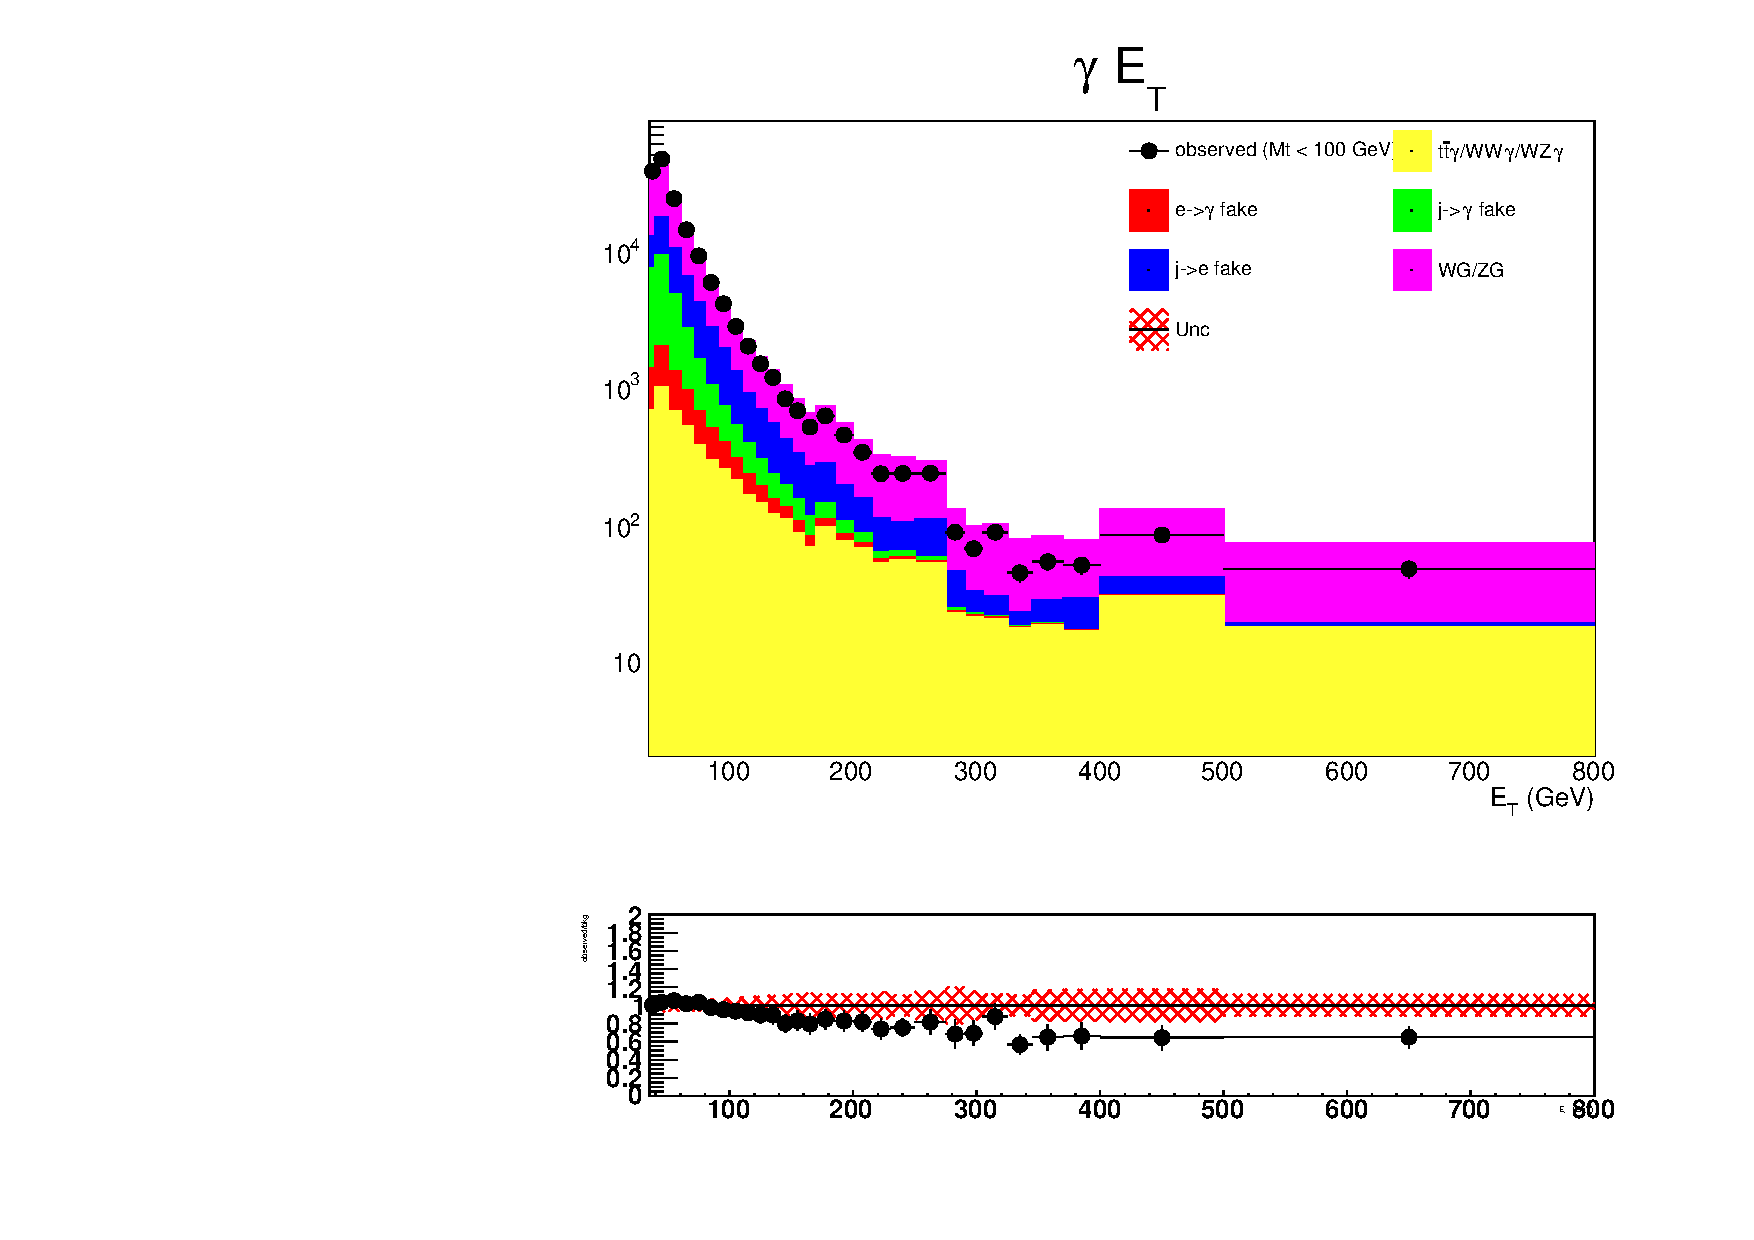
\includegraphics[width=0.45\textwidth]{Figures/VALIDNOCOR_mg_2016ReMiniAOD_pt.pdf} \\
    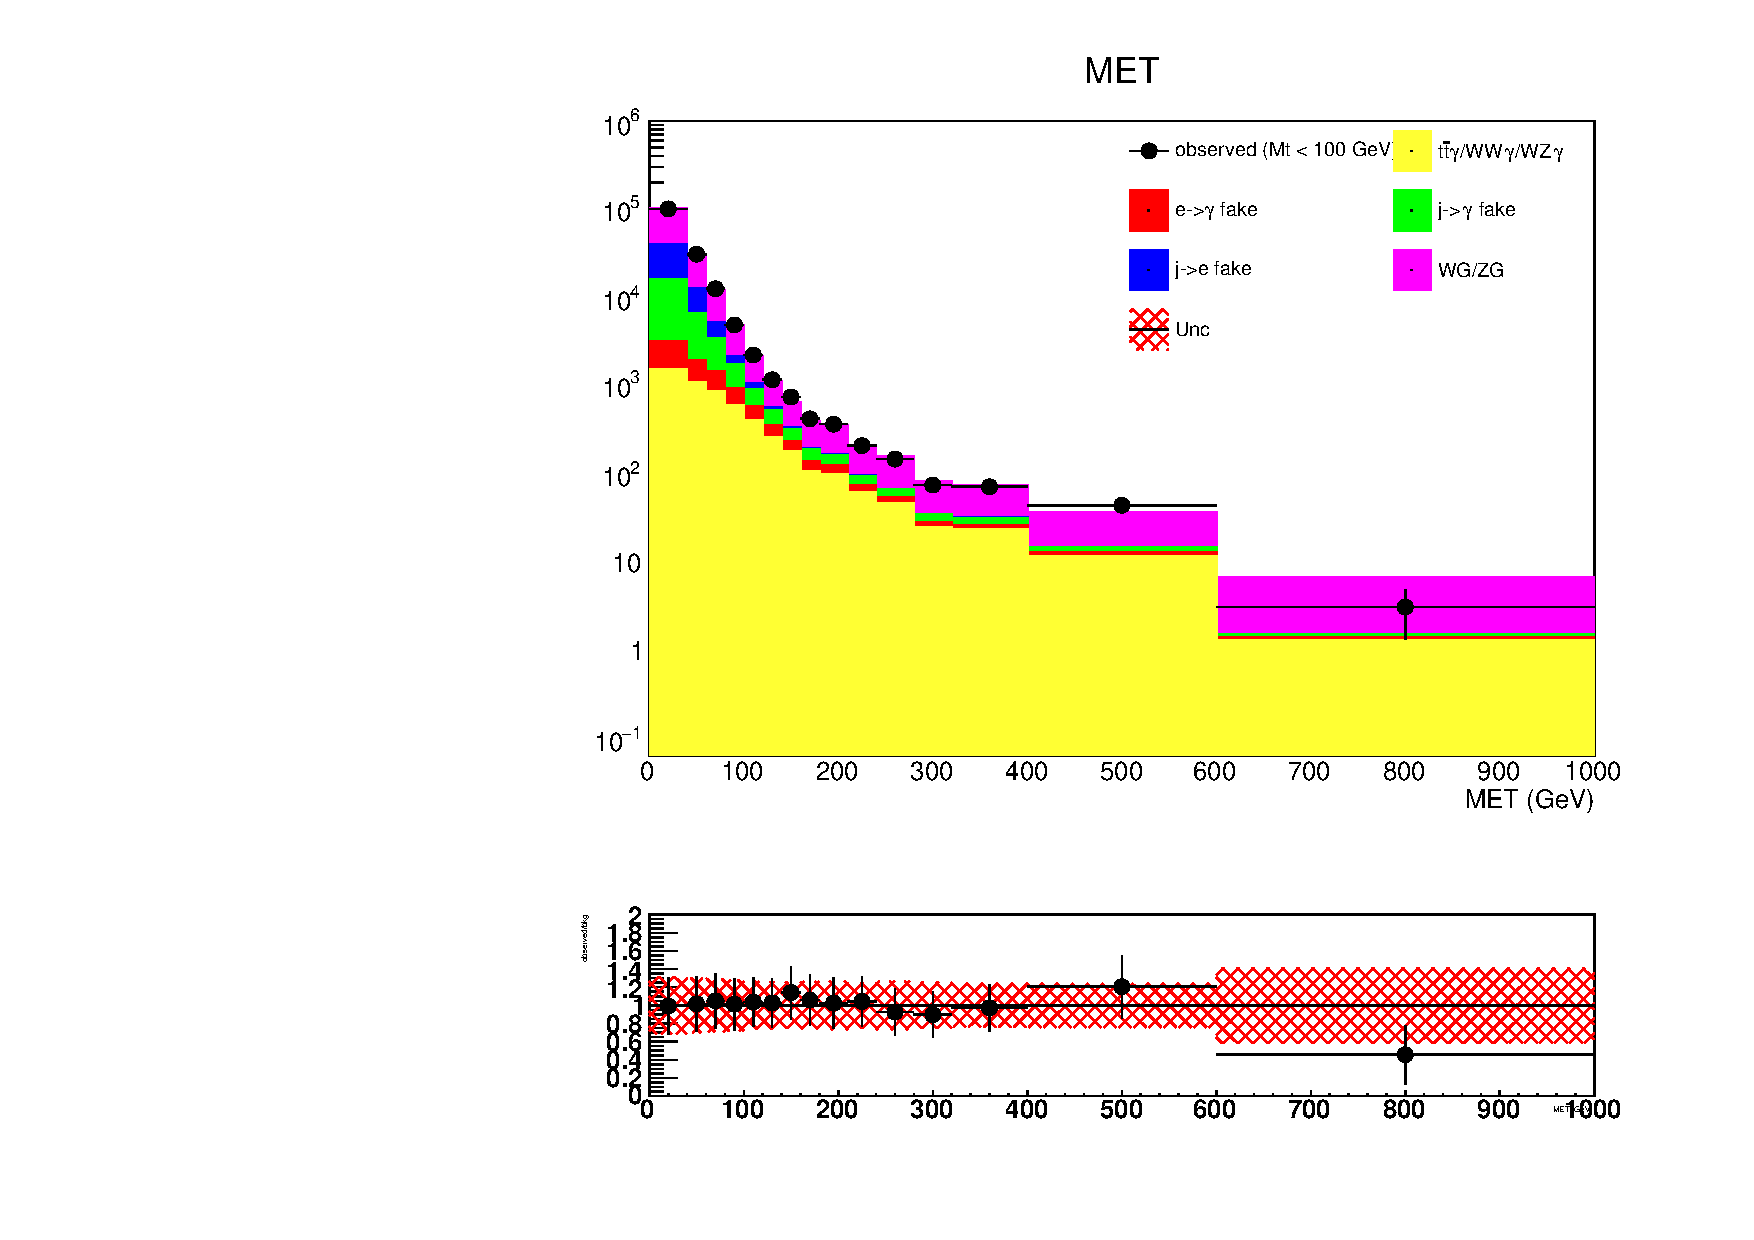
\includegraphics[width=0.45\textwidth]{Figures/VALID_mg_2016ReMiniAOD_met.pdf}
    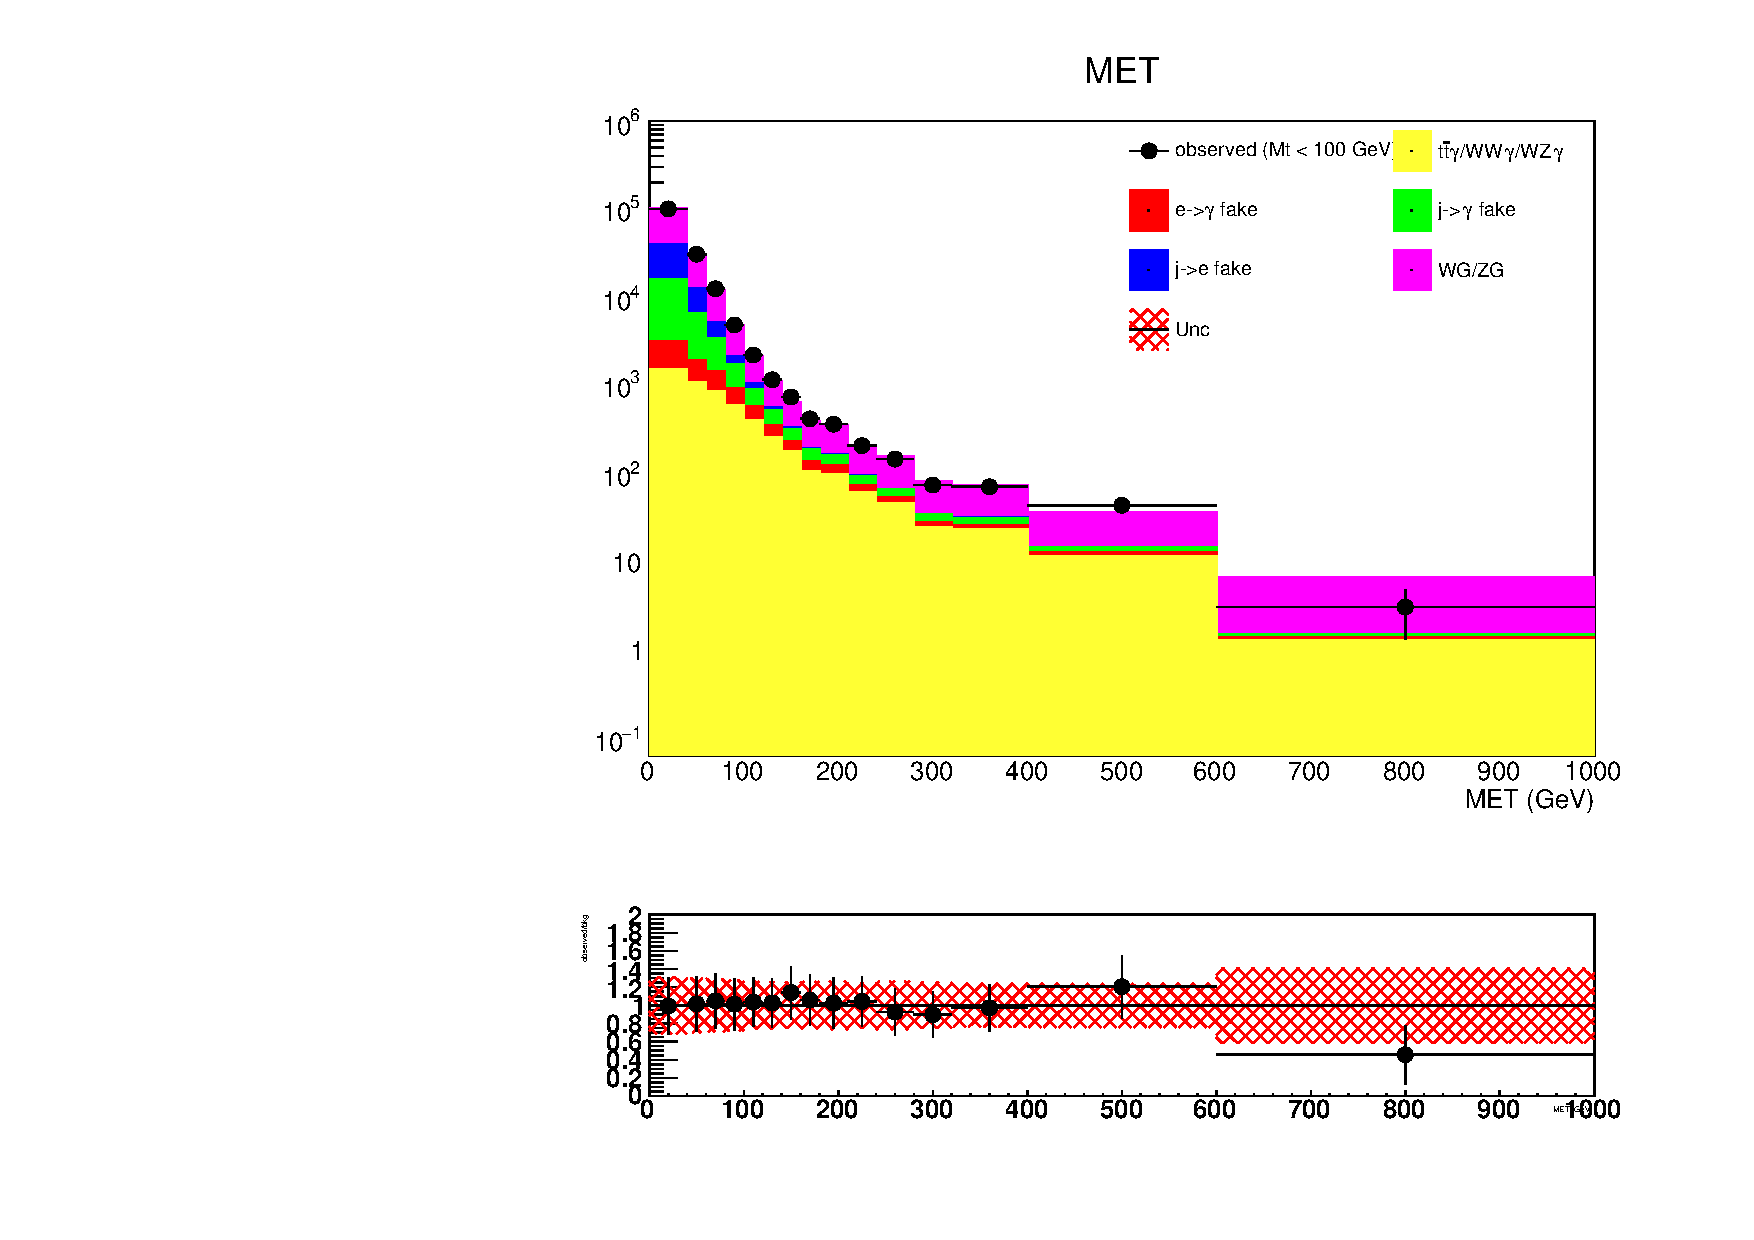
\includegraphics[width=0.45\textwidth]{Figures/VALID_mg_2016ReMiniAOD_met.pdf}
  \caption{$p_T^{miss}$ (left) and photon $p_T$ distributions of the data and background predictions in the validation region. Top: no ISR reweighting applied, bottom: with ISR corrections. }
  \label{fig:apen-withcorr}
\end{figure}

\end{document}
